\begin{frame}
~\\
{\blank
\underline{RECAP:}\\
$ A\in\mathbb{F}^{n\times n} $
\begin{align*}
&\lambda\in\mathbb{C}~\text{eigenvalue}~~:\Leftrightarrow~~\exists v\neq 0:~Av=\lambda v\\
&(\lambda_i, v_i),~Av_i=\lambda_i v_i\\
&V:=\begin{pmatrix}
|&~&|\\
v_1&\dots&v_n\\
|&~&|
\end{pmatrix},~
\Lambda:=\begin{pmatrix}
\lambda_1&~&0\\
~&\ddots&~\\
0&~&\lambda_n
\end{pmatrix}\\
&AV=V\Lambda\\
&A~\text{is diagonalizable}~~:\Leftrightarrow~~\exists V\in GL_n(\mathbb{F}),~\Lambda~\text{diagonal}:~A=V\Lambda V^{-1}~(V^{-1}AV=\Lambda)
\end{align*}
\underline{Powers of a matrix:}
\begin{align*}
&A\cdot A=V\Lambda\underbrace{V^{-1}V}_{I}\Lambda V^{-1}=V\Lambda^2V^{-1}~~(\Lambda^2:=\begin{pmatrix}
\lambda_1^2&~&0\\
~&\ddots&~\\
0&~&\lambda_n^2
\end{pmatrix})\\
k\in\mathbb{N}:~&A^k=V\Lambda^kV^{-1}\\
s\in (0,1):~&A^s:=V\Lambda^sV^{-1}~\rightarrow~\text{may be dense even if}~A~\text{is sparse}\\
&\begin{pmatrix}
D(f):=f''=(\frac{d}{dx})^2f\\
D(\sin):=(\sin')'=-\sin
\end{pmatrix}
\frac{1}{C(h)}\begin{pmatrix}
2&-1&~&0\\
-1&\ddots&\ddots&~\\
~&\ddots&\ddots&-1\\
0&~&-1&2
\end{pmatrix}~\rightarrow~\text{many zeros}~\Leftrightarrow~\text{sparse matrix}
\end{align*}
}
\end{frame}

\begin{frame}
~\\
{\blank
\begin{align*}
\begin{pmatrix}
/&/&/\\
/&/&/\\
/&/&/
\end{pmatrix}
\begin{pmatrix}
x_1\\\vdots\\x_n
\end{pmatrix}
=\begin{pmatrix}
b_1\\\vdots\\b_i\\\vdots\\b_n
\end{pmatrix}~\leftarrow~\text{i-th},~~~~~
P_1 \frac{1}{n} P_2 = \text{dense matrix}\\
\textcolor{orange}{(A\in\mathbb{C}^{n\times n}~\text{is called hermitation}~:\Leftrightarrow~~\bar{A}^T=A)}
\end{align*}
\underline{Eigendecomposition of symmetric matrices:}\\
$A\in\mathbb{R}^{n\times n}$ symmetric $\Rightarrow~~A=Q\Lambda Q^T$\\
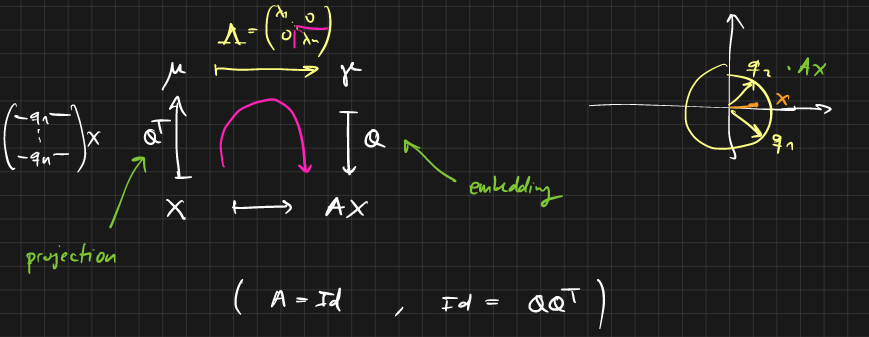
\includegraphics[width=0.5\textwidth]{\PathToMedia/eigendecomposition.png}
}
\end{frame}

\begin{frame}
~\\
{\blank
\underline{Eigenvalue Algorithms:}
\begin{itemize}\blank
	\item [1)]
	Direct method: $n=2,3$
	\begin{itemize}
		\item [i)]
		Root finding problem: $ \rightarrow~\sigma(A) $\\
		$ \chi_{A}(\lambda)=~\text{det}(A-\lambda I)=0 $
		\item [ii)]
		Solving linear system: $ \rightarrow $ eigenvectors\\
		$ Av=\lambda v~~\Leftrightarrow~~(A-\lambda I)v = 0 $
	\end{itemize}
	\item [2)]
	Power method:\\
	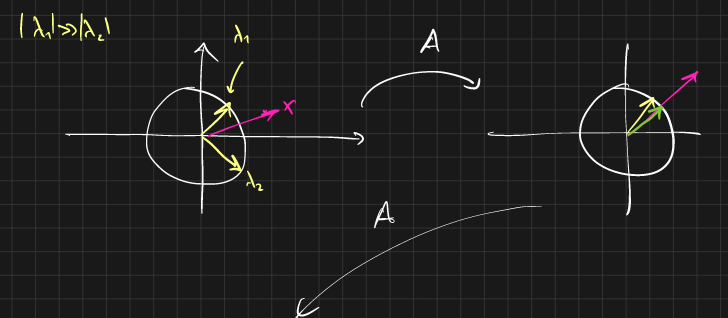
\includegraphics[width=0.7\textwidth]{\PathToMedia/power_method_recap.png}
	\begin{align*}
	&A\dots AAAx_0=A^kx_0=x^k\\
	&A~\text{symmetric},~A=Q\Lambda Q^T\\
	A^kx_0&=\sum_{i=1}^n \lambda_i^k x_0^T q_i \begin{pmatrix}
	|\\q_i\\|
	\end{pmatrix}
	=\lambda_1^k x_0^T q_1 \begin{pmatrix}
	|\\q_1\\|
	\end{pmatrix}
	+\sum_{i=1}^n \lambda_i^k x_0^T q_2 \begin{pmatrix}
	|\\q_2\\|
	\end{pmatrix}
	\end{align*}
\end{itemize}
}
\end{frame}

\begin{frame}
	~\\
	{\blank
		\underline{RECAP:}\\
		\underline{Eigenvectors and -values}\\
		Let $A\in\mathbb{F}^{n\times n}$\\
		eigenvectors= vectors that do not change direction if multiplied with;\\
		$\rightarrow$ they are only scaled by a certain factor (=eigenvalue)
		\begin{align*}
		\lambda\in\mathbb{C}~\text{is an eigenvalue of}~A~~:\Leftrightarrow~~\exists~v\in\mathbb{F}^n\setminus\{0\}:~&Av=\lambda v\\
		(\lambda\in\sigma(A))~~~~~~~\Leftrightarrow~~&Av-\lambda v=0\\
		\Leftrightarrow~~&(A-\lambda I)v=0\\
		\Leftrightarrow~~&v\in\text{ker}(A-\lambda I)\supsetneq\{0\}\\
		\Leftrightarrow~~&\text{det}(A-\lambda I) = 0~~\forall\lambda\in\sigma(A)
		\end{align*}
		\underline{Examples:}\\
		1) PageRank = eigenvector to the eigenvalue 1\\
		2)$A=\begin{pmatrix}2&1\\1&2\end{pmatrix}$ look slide above
	}
\end{frame}